% ============================================================
%  CHAPTER 2: LITERATURE REVIEW AND PROBLEM BACKGROUND
% ============================================================

\chapter{LITERATURE REVIEW AND PROBLEM BACKGROUND}
\label{chap:literature_review}

\section{Quantum Vulnerability of Classical Cryptosystems}
\label{sec:quantum_vulnerability}

Contemporary secure communications protocols rely almost universally on public-key cryptosystems founded on the computational hardness of mathematical problems in number theory:
\begin{enumerate}[label=(\alph*)]
    \item Integer Factorization Problem (IFP): The foundation of RSA~\cite{alagic2022nist}, wherein finding prime factors $p, q$ of $N = p \cdot q$ requires sub-exponential time $\mathcal{O}\big(\exp(c \cdot (\ln N)^{1/3} (\ln \ln N)^{2/3})\big)$ via the General Number Field Sieve (GNFS).
    \item Discrete Logarithm Problem (DLP) and Elliptic Curve DLP (ECDLP): The foundation of Diffie-Hellman (DH) and ECDH (e.g., Curve25519)~\cite{stallings2022cryptography}.
\end{enumerate}

In 1994, Peter Shor formulated a quantum algorithm utilizing quantum Fourier transforms that computes the order of an element in a finite cyclic group in polynomial time~\cite{mavroeidis2022impact}:
\begin{equation}
\mathcal{O}\left( (\log N)^2 \cdot (\log \log N) \cdot (\log \log \log N) \right)
\end{equation}
Consequently, a Cryptographically Relevant Quantum Computer (CRQC) running Shor's algorithm completely breaks RSA-2048, RSA-4096, and 256-bit elliptic curve schemes in fractions of a second. Symmetric ciphers such as AES are affected by Grover's quantum search algorithm~\cite{mavroeidis2022impact,cisa2023postquantum}, which provides a quadratic speedup from $\mathcal{O}(2^n)$ to $\mathcal{O}(2^{n/2})$. Thus, AES-128 is reduced to 64 bits of security, whereas AES-256 retains 128 bits of post-quantum security, satisfying top-secret security parameters.

\section{NIST Post-Quantum Cryptography Standardization}
\label{sec:nist_standardization}

In response to the quantum threat, the National Institute of Standards and Technology (NIST) conducted an eight-year international competition evaluating post-quantum candidates across lattice-based, code-based, and isogeny-based mathematical paradigms. In August 2024, NIST released the finalized Federal Information Processing Standards (FIPS):
\begin{enumerate}
    \item FIPS 203: ML-KEM (Module-Lattice-Based Key-Encapsulation Mechanism, derived from CRYSTALS-Kyber)~\cite{nist_fips_203}.
    \item FIPS 204: ML-DSA (Module-Lattice-Based Digital Signature Algorithm, derived from CRYSTALS-Dilithium)~\cite{nist_fips_204}.
    \item FIPS 205: SLH-DSA (Stateless Hash-Based Digital Signature Algorithm, derived from SPHINCS+)~\cite{nist_fips_205}.
\end{enumerate}

ML-KEM and ML-DSA are grounded in the hardness of the Module Learning with Errors (M-LWE) and Module Short Integer Solution (M-SIS) problems over polynomial rings $\mathcal{R}_q = \mathbb{Z}_q[X]/(X^{256} + 1)$ with modulus $q = 3329$. ML-KEM-1024 provides NIST Security Level 5 (equivalent to brute-forcing AES-256) with public keys of 1,568 bytes, ciphertexts of 1,568 bytes, and shared secrets of 32 bytes, achieving microsecond-level encapsulation on modern microprocessors.

\section{Android VPN Architecture and Kernel Socket Protection}
\label{sec:android_vpn_arch}

On the Android platform, VPN applications operate in user space via the managed \texttt{android.net.VpnService} API~\cite{android_vpnservice_docs}. The framework exposes a virtual TUN network interface that captures outgoing system-wide IP datagrams. A fundamental challenge in user-space VPN design is avoiding the catastrophic routing loop:
\begin{equation}
\text{App Packet} \to \text{TUN} \to \text{VPN Service} \to \text{Socket} \to \text{Routing Table} \to \text{TUN} \to \dots
\end{equation}
To eliminate this feedback loop, Android provides the kernel method \texttt{protect(int socketFd)} or \texttt{protect(Socket socket)}. The system call applies the \texttt{SO\_\allowbreak BINDTODEVICE} or \texttt{SO\_MARK} socket option at the Linux kernel level, explicitly directing all encapsulated VPN transport packets to bypass the TUN routing table and egress directly through the physical network adapter (e.g., \texttt{wlan0} or cellular \texttt{rmnet\_data0}).

\begin{table}[htbp]
  \centering
  \small
  \caption{Architectural Comparison: Desktop Prototype vs. Native Android Application.}
  \label{tab:python_vs_android_architecture}
  \begin{tabularx}{\linewidth}{@{}p{3.2cm}YY@{}}
    \toprule
    \textbf{Dimension} & \textbf{Desktop Python Prototype} & \textbf{Native Android Application} \\
    \midrule
    Execution Runtime & CPython 3.12 interpreter & Android Runtime (ART) Ahead-Of-Time (AOT) \\
    Language Stack & Python with C bindings & Kotlin 1.9 with Jetpack Compose (Material 3) \\
    TUN Device Access & Direct Linux \texttt{/dev/net/tun} (Root) & Sandboxed \texttt{android.net.VpnService} \\
    Socket Protection & Manual policy routing / \texttt{ip rule} & Native OS \texttt{protect(socket)} system call \\
    Process Lifecycle & Persistent CLI daemon & Foreground Service with active Notification \\
    Cryptography Engine & Dynamic C-bindings (\texttt{liboqs}) & Pure-Kotlin lattice arithmetic with SHA-3 \\
    State Management & Global variables \& console logs & Reactive MVVM with Kotlin Coroutines \& \texttt{StateFlow} \\
    \bottomrule
  \end{tabularx}
\end{table}

\section{Comparative Survey of Existing VPN Solutions}
\label{sec:comparative_survey}

Table~\ref{tab:vpn_solutions_matrix} compares existing mainstream commercial and academic VPN implementations against QuantumSafe VPN across key cryptographic and platform dimensions.

\begin{table}[htbp]
  \centering
  \footnotesize
  \setlength{\tabcolsep}{3.5pt}
  \caption{Comprehensive Technical Comparison of Virtual Private Network Implementations.}
  \label{tab:vpn_solutions_matrix}
  \begin{tabularx}{\linewidth}{@{}p{2.3cm}p{2.3cm}p{2.2cm}p{1.9cm}Y@{}}
    \toprule
    \textbf{Solution} & \textbf{Key Exchange} & \textbf{Data Cipher} & \textbf{Quantum Safe?} & \textbf{Key Limitations} \\
    \midrule
    OpenVPN & TLS (ECDHE / RSA) & AES-256-GCM & No & High CPU overhead; large codebase ($>100$k lines) \\
    WireGuard & Noise (Curve25519) & ChaCha20-Poly1305 & No & Classical DH; vulnerable to HNDL quantum archiving \\
    StrongSwan & IKEv2 (DH / ECDH) & AES-GCM / CBC & No & Complex configuration; pre-quantum key exchange \\
    Tailscale & WireGuard (Curve25519) & ChaCha20-Poly1305 & No & Proprietary coordination server; pre-quantum \\
    QuantumSafe VPN & ML-KEM-1024 & AES-256-GCM & Yes (FIPS 203) & Full post-quantum security with native Android UI \\
    \bottomrule
  \end{tabularx}
\end{table}

\section{Requirements Analysis and Operational Specifications}
\label{sec:requirements_analysis}
\label{chap:requirements}

The system requirements formalize both the functional capabilities and rigorous non-functional operational boundaries demanded by secure mobile VPN communications.

\subsection{Functional Requirements Specification}
\label{sec:functional_requirements}

The functional requirements define the explicit operational capabilities of the QuantumSafe VPN system:
\begin{itemize}[leftmargin=1.8em, itemsep=4pt]
    \item \textbf{FR-1 (Post-Quantum Handshake Negotiation):} The client and gateway must execute an authenticated key exchange using ML-DSA-65 (FIPS 204) and ML-KEM-1024 (FIPS 203) without exposing sensitive keys.
    \item \textbf{FR-2 (Dynamic Virtual IP Leasing):} The server must lease a private IPv4 address from the \texttt{10.8.0.0/24} subnet upon successful handshake authentication.
    \item \textbf{FR-3 (Full Tunnel IP Encapsulation):} The Android \texttt{VpnService} must capture all outbound device IPv4 traffic (\texttt{0.0.0.0/0}) and route it into the encrypted tunnel.
    \item \textbf{FR-4 (Symmetric Encryption with Replay Protection):} All payload frames must be encrypted with hardware-accelerated AES-256-GCM authenticated encryption utilizing a 64-bit monotonically increasing sequence counter.
    \item \textbf{FR-5 (DNS Leak Prevention):} Outbound DNS requests must be forcefully bound to verified recursive resolvers (\texttt{1.1.1.1} and \texttt{8.8.8.8}) through the encrypted tunnel.
    \item \textbf{FR-6 (Connection Management and Recovery):} The application must support manual connect/disconnect toggling and automatic graceful resource cleanup upon network drops.
\end{itemize}

\subsection{Non-Functional Requirements Specification}
\label{sec:non_functional_requirements}

The non-functional requirements enforce performance, security, and mobile usability constraints:
\begin{itemize}[leftmargin=1.8em, itemsep=4pt]
    \item \textbf{NFR-1 (Post-Quantum Security Level):} The system must deliver NIST Security Level 5 ($>256$ bits of classical and quantum hardness).
    \item \textbf{NFR-2 (Handshake Latency):} Handshake completion over 4G/5G/Wi-Fi links must terminate in under 150\,ms under nominal conditions.
    \item \textbf{NFR-3 (Memory Footprint):} The Android background service must maintain resident memory consumption below 60\,MB.
    \item \textbf{NFR-4 (Battery Efficiency):} Zero active CPU spinning during idle connection states; non-blocking asynchronous socket polling.
\end{itemize}

\section{Trust Boundaries, Threat Modeling, and Traceability Matrix}
\label{sec:threat_boundaries_rtm}

\subsection{Use Case Analysis}
Figure~\ref{fig:use_case_diagram} depicts the system use-case diagram illustrating interactions between the Mobile User, Cryptographic Subsystem, and Linux VPN Gateway.

\begin{figure}[htbp]
  \centering
  \resizebox{0.68\linewidth}{!}{%
  \begin{tikzpicture}[
    actor/.style={draw=vpnblue, line width=1pt, rounded corners=2pt, minimum width=2.4cm, minimum height=1cm, align=center, fill=codebg},
    usecase/.style={draw=vpnblue!80!black, line width=0.8pt, ellipse, minimum width=3.2cm, minimum height=0.9cm, align=center, fill=white},
    arrow/.style={-Latex, thick, draw=darkcharcoal}
  ]
    \draw[dashed, color=mutedgrey, line width=0.8pt, fill=codebg!40] (-0.5,-3.8) rectangle (6.5,1.2);
    \node[anchor=north west, font=\bfseries\footnotesize, color=darkcharcoal] at (-0.3,1.0) {QuantumSafe VPN System Boundary};
    
    \node[actor] (user) at (-3,-1.3) {\textbf{Mobile User}};
    \node[actor] (gateway) at (9,-1.3) {\textbf{VPN Gateway}};
    
    \node[usecase] (uc1) at (3,0.3) {UC-01: Initiate PQC Connection};
    \node[usecase] (uc2) at (3,-0.8) {UC-02: Authenticate Identity};
    \node[usecase] (uc3) at (3,-1.9) {UC-03: Route Encrypted Traffic};
    \node[usecase] (uc4) at (3,-3.0) {UC-04: Terminate Session};
    
    \draw[arrow] (user) -- (uc1);
    \draw[arrow] (user) -- (uc2);
    \draw[arrow] (user) -- (uc3);
    \draw[arrow] (user) -- (uc4);
    
    \draw[arrow] (gateway) -- (uc1);
    \draw[arrow] (gateway) -- (uc2);
    \draw[arrow] (gateway) -- (uc3);
  \end{tikzpicture}
  }
  \caption[Use Case Diagram of QuantumSafe VPN System]{Use Case Diagram: This figure illustrates the operational interactions between the mobile client user, cryptographic subsystems, and the Linux VPN gateway.}
  \label{fig:use_case_diagram}
\end{figure}

\subsection{Architectural Trust Boundaries}
Figure~\ref{fig:threat_model_concept} illustrates the architectural trust boundaries dividing the trusted mobile execution perimeter from the untrusted transit carrier network and the trusted security gateway.

\begin{figure}[htbp]
  \centering
  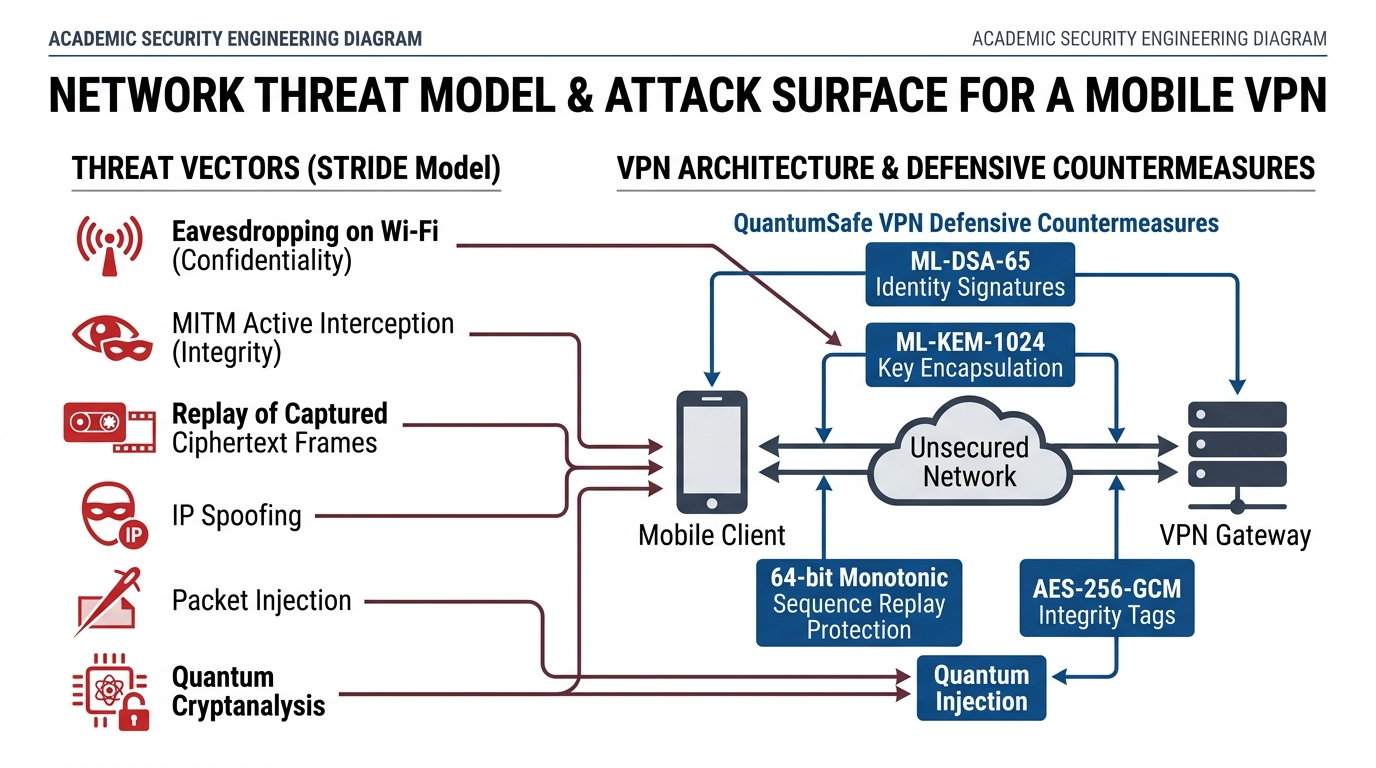
\includegraphics[width=0.88\linewidth,height=0.30\textheight,keepaspectratio]{figures/threat_model_concept.jpg}
  \caption[Architectural Trust Boundaries and Network Threat Vectors]{Architectural Trust Boundaries: This figure illustrates the security perimeter between the trusted Android client runtime, untrusted transit carrier infrastructure, and the hardened gateway.}
  \label{fig:threat_model_concept}
\end{figure}

\subsection{Requirement Traceability Matrix}
Table~\ref{tab:rtm_matrix} provides the Requirement Traceability Matrix (RTM) linking requirements to design and verification modules.

\begin{table}[htbp]
  \centering
  \footnotesize
  \setlength{\tabcolsep}{3pt}
  \caption{Requirement Traceability Matrix (RTM).}
  \label{tab:rtm_matrix}
  \begin{tabularx}{\linewidth}{@{}p{1.4cm}p{3.0cm}p{3.5cm}Yp{1.9cm}@{}}
    \toprule
    \textbf{Req ID} & \textbf{Requirement Name} & \textbf{Design Element} & \textbf{Implementation} & \textbf{Test Case} \\
    \midrule
    FR-01 & PQC Handshake & Stage 1--4 Handshake FSM & \texttt{PqcEngine.kt} & TC-SEC-01 \\
    FR-02 & Dynamic IP Lease & IP Pool Subsystem & \texttt{ip\_pool.py} & TC-INT-02 \\
    FR-03 & Full Tunnel Routing & VpnService TUN Capture & \texttt{QuantumSafe}\allowbreak\texttt{VpnService} & TC-VPN-01 \\
    FR-04 & AES-256-GCM AEAD & Frame Crypto Engine & \texttt{classical.py} & TC-SEC-03 \\
    FR-05 & Anti-Replay Guard & 64-bit Sequence Counter & \texttt{PqcEngine.kt} & TC-SEC-04 \\
    FR-06 & DNS Leak Defense & Explicit Resolver Binding & \texttt{VpnService.}\allowbreak\texttt{Builder} & TC-NET-01 \\
    \bottomrule
  \end{tabularx}
\end{table}
